\section{Controllers}

In an imitation learning setting, there are two controllers involved: an \emph{omniscient} controller, which performs the desired task with perfect knowledge of the environment, and a \emph{learned} controller, which is trained to imitate the behaviour of the omniscient controller.

\subsection{Omniscient controller}

We implemented a controller from the literature that simultaneously controls position and orientation of the robot toward a certain goal pose~\cite{park2011smooth}.

We chose this particular controller because it promised smooth and intuitive 
trajectories, which globally converge to arbitrary goal poses without 
singularities, from any initial pose. Furthermore, this specific formulation 
makes it easy to impose limits on the velocity, acceleration and jerk of the 
resulting paths, ensuring that they would be physically realizable if executed
on a real robot.

The control law is described in an egocentric polar coordinate system, relative to the current pose of the robot. The control variables are the linear $v$ and angular $\omega$ velocities. Given a target pose $T$, the state of the robot is expressed as the triple $(r, \theta, \delta)$, where $r$ is the Euclidean distance from the target position; $\theta \in (-\pi, \pi]$ the target orientation with respect to the line of sight from the robot to the target position; $\delta \in (-\pi, \pi]$ the vehicle orientation with respect to the line of sight, as shown in Figure~\ref{fig:egocentric-coordinates}.

It can be seen that $(r, \theta)$ completely identify the position of the robot, while $\delta$ identifies its orientation. In this formulation, moving the robot to the target pose corresponds to bringing the state to the origin, $(r, \theta, \delta) = (0, 0, 0)$.

\begin{figure}[htbp]
	\centerline{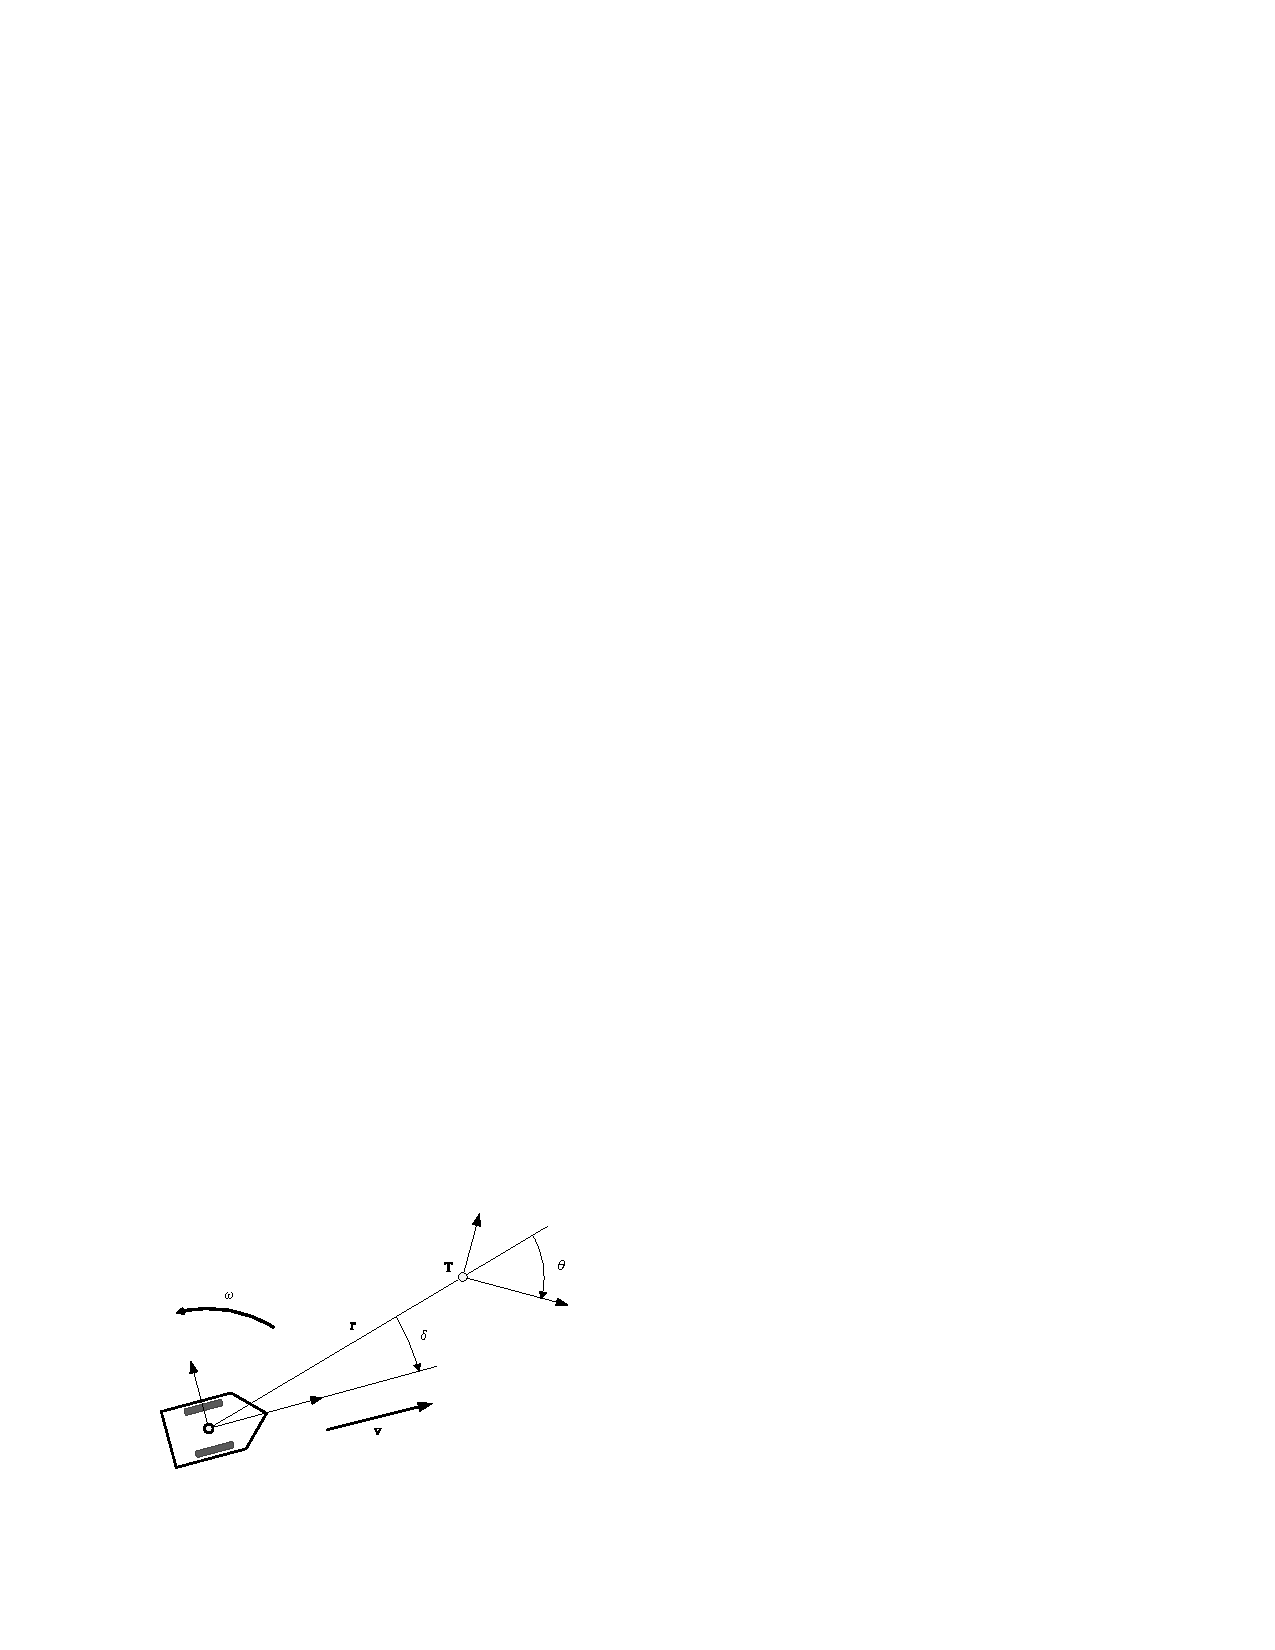
\includegraphics[width=\columnwidth]{controller/egocentric-coordinates}}
	\caption{Egocentric polar coordinate system, relative to the current pose of the robot.}
	\label{fig:egocentric-coordinates}
\end{figure}

Assuming initially the linear velocity $v$ is nonzero positive and given (although not constant), the authors show that the angular velocity $\omega$ only influences $\delta$ directly, which in turn influences $(r, \theta)$. As such, the control problem is decomposed in a slow and a fast subsystem.

The slow subsystem first computes a reference orientation $\hat{\delta}$ to steer the robot toward the origin:
\begin{IEEEeqnarray}{l}
	\hat{\delta} = \arctan(-k_1 \theta)
\end{IEEEeqnarray}

The fast subsystem then controls the angular velocity $\omega$ to bring the current orientation $\delta$ toward the reference orientation $\hat{\delta}$ computed by the slow subsystem (somewhat confusingly, the original paper uses $\delta$ for both the current and reference orientations):
\begin{IEEEeqnarray}{l}
	\omega = -\frac{v}{r} [
		k_2 (\delta - \underbrace{\arctan(-k_1 \theta)}_{\hat{\delta}}) +
		(1 + \underbrace{\frac{k_1}{1 + (k_1\theta)^2}}_{-\dot{\hat{\delta}}})\sin\theta
	] \notag \\
	\label{eq:angular-vel}
\end{IEEEeqnarray}

It can be seen from \eqref{eq:angular-vel} that there is a linear relation between $v$ and $\omega$. In particular, $\, \omega = \kappa(r, \theta, \delta) \, v$ where $\kappa$ is the curvature of the resulting path. It is possible to rewrite \eqref{eq:angular-vel}, such that
\begin{IEEEeqnarray}{l}
	\kappa = -\frac{1}{r} [k_2 (\delta - \hat{\delta}) + (1 - \dot{\hat{\delta}})\sin\theta]
	\label{eq:curvature}
\end{IEEEeqnarray}
which implies that the shape of the path does not depend on the choice of $v$. To ensure a smooth and comfortable trajectory, the authors suggest to choose $v$ so that $v \rightarrow 0$ as $\kappa \rightarrow \pm\infty$ and $v \rightarrow v_\text{max}$ as $\kappa \rightarrow 0$:
\begin{IEEEeqnarray}{l}
	v = \frac{v_\text{max}}{1 + \beta |\kappa(r, \theta, \delta)|^\lambda}
	\label{eq:linear-vel}
\end{IEEEeqnarray}

As written, the control law has a singularity as $r \rightarrow 0$, in other words when the robot approaches the target. We address this problem as suggested in the original paper, by setting $v = k_3 r$ in the neighbourhood of $r = 0$:
\begin{IEEEeqnarray}{l}
	v' = \min(v, k_3 r)
	\label{eq:final-linear-vel}
\end{IEEEeqnarray}

In the equations above $k_1 > 0$, $k_2 > 0$, $k_3 > 0$, $\beta > 0$ and $\lambda > 1$ are design parameters. Figure~\ref{fig:omniscient-trajectories} shows some trajectories generated by this controller, obtained with parameters $k_1 = 1$, $k_2 = 3$, $k_3 = 2$, $\beta = 0.4$ and $\lambda = 2$.

\begin{figure}[htbp]
	\centerline{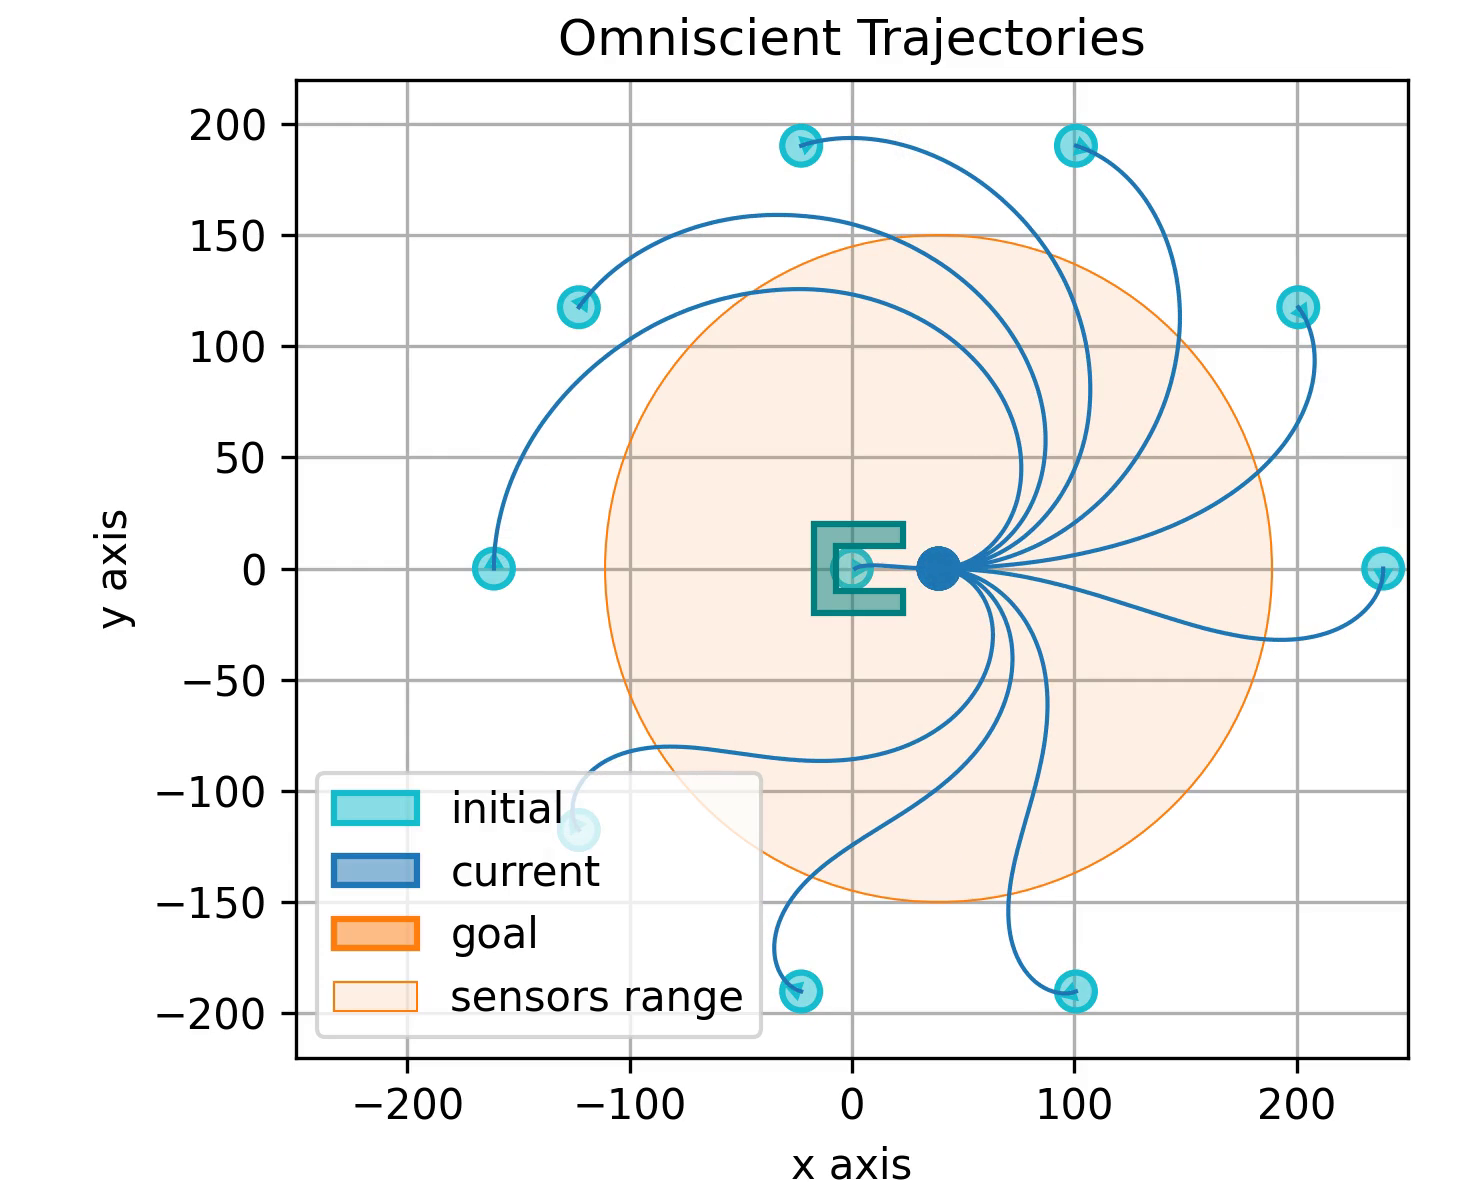
\includegraphics[width=.8\columnwidth]{controller/demo-circle-omniscient-trajectories}}
	\caption{Trajectories of the omniscient controller from 9 initial poses.}
	\label{fig:omniscient-trajectories}
\end{figure}

Finally, we implemented support for reverse gear as suggested by the authors: by simultaneously flipping the orientation of both the robot and the target when $v$ is negative. 

We use the reverse gear to teach the learned controller how to behave when it overshoots the target. This normally never happened with the omniscient controller, so the neural network wouldn't know what to do if it didn't stop precisely over the goal. We used an augmentation technique to ensure that this situation would be present in the training set: we made the robot move in reverse if its initial position was inside a region in front of the goal (i.e. between the arms of the object in Figure~\ref{fig:omniscient-trajectories}).

\subsection{Learned controller}

Our learned controller is implemented as an end-to-end neural network, which 
receives the sensor inputs and produces commands for the motors. 
Section~\ref{sec:models} will describe the specific architectures that we used.
